\section{Valutazione sperimentale delle varianti proposte}
Per tutte le simulazioni è stata usata la configurazione nella \textbf{Tabella \ref{configs}} facendo variare ogni volta il parametro \textit{iaTime} con cui si regola il traffico in rete, infatti, i nodi generano un pacchetto DATA ogni \textit{iaTime} secondi.\\
I risultati presentati sono mediati su un numero di run sufficiente a fornire un intervallo di confidenza del 95\% con una precisione del 5\%. \\
Per ciascuna metrica viene presentata la media  ottenuta nelle simulazioni effettuate. \\
Si precisa che sono inclusi nei risultati anche i consumi energetici dovuti alla fase di \textit{interest dissemination}.


\subsection{Auto-WakeUp}
\textit{1) TX Time}: come mostrato in \textbf{Figura \ref{fig:TXTime_1}}, il tempo medio che le varie antenne di WakeUp passano in TX diminuisce in modo significativo all'aumentare del traffico in rete. Questo risultato giustifica anche quanto è possibile vedere in \textbf{Figura \ref{fig:EnergySpent_1}} in quanto  i vari nodi che ricoprono il ruolo di \textit{receiver}, e che quindi svolgono la funzione di relay per un determinato pacchetto, non inviano più il WakeUp message prima del CTS e in questo modo si vanno a risparmiare \textit{n*m} invii nel caso in cui si hanno \textit{n} potenziali nodi relay e \textit{m} pacchetti data da inviare. In questo caso i miglioramenti sono costantemente tra il 72\% e il 73\%.
\\\\
\textit{2) Energy Consuption}: come mostrato in \textbf{Figura \ref{fig:EnergySpent_1}}, si ha un miglioramento nell'energia complessiva consumata dalla rete alla fine della simulazione. In particolare si ottiene un miglioramento maggiore all'aumentare del traffico in rete, infatti, l'energia consumata diminuisce di circa 7\% nel caso in cui si genera un data packet ogni 50 secondi (circa 65 pacchetti in totale), mentre diminuisce di circa 11\% nel caso in cui si genera un data packet ogni 2 secondi (circa 1700 pacchetti in totale).
\\\\
\textit{3) End-to-End Latency}: come mostrato in \textbf{Figura \ref{fig:Latency_1}}, la latenza è un parametro che ne risente, invece, negativamente. Questo può essere dovuto al fatto che, svegliandosi da solo, il nodo mittente non riesca sempre a ricevere il primo pacchetto CTS per cui deve aspettare il prossimo. Tuttavia, la variante proposta risulta sì più lenta, ma questo ritardo varia da un massimo di 8 millisecondi fino ad un minimo di 6 millisecondi per cui non risulta essere un ritardo particolarmente problematico.
\\\\
\textit{4) Packet Delivery Ratio}: come mostrato in \textbf{Figura \ref{fig:PDR_1}}, il PDR è anch'esso un parametro che risente in modo negativo delle modifiche apportate con autoWakeUp. Dalle simulazioni, così come dal grafico, si evince una perdita di circa lo 0.5\% in più rispetto alla versione base del protocollo nel caso iaTime è 2. Nonostante il PDR più basso, la variante proposta riesce comunque a consegnare sempre almeno il 99.3\% dei pacchetti generati (contro il 99.8\% del base GreenWUP), risultato comunque accettabile nonostante la piccola perdita di qualità.

\begin{figure}[H]
  \begin{subfigure}[t]{0.49\linewidth}
    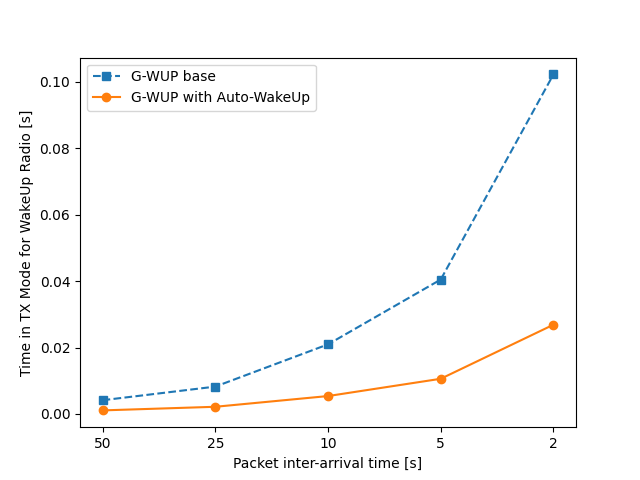
\includegraphics[width=1.1\linewidth]{Contents/Images/graphs/autoWakeUp/tx_time.png}
    \caption{TX Time for the WUR}
    \label{fig:TXTime_1}
  \end{subfigure}
  \begin{subfigure}[t]{0.49\linewidth}
    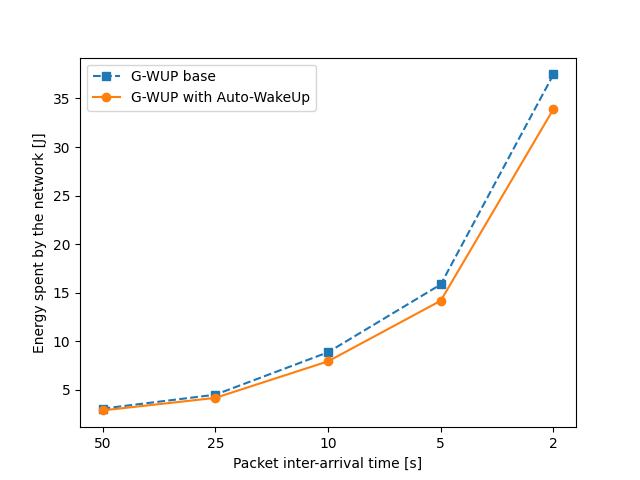
\includegraphics[width=1.1\linewidth]{Contents/Images/graphs/autoWakeUp/energySpent.png}
    \caption{Energy Consuption}
    \label{fig:EnergySpent_1}
  \end{subfigure}
  \begin{subfigure}[t]{0.49\linewidth}
    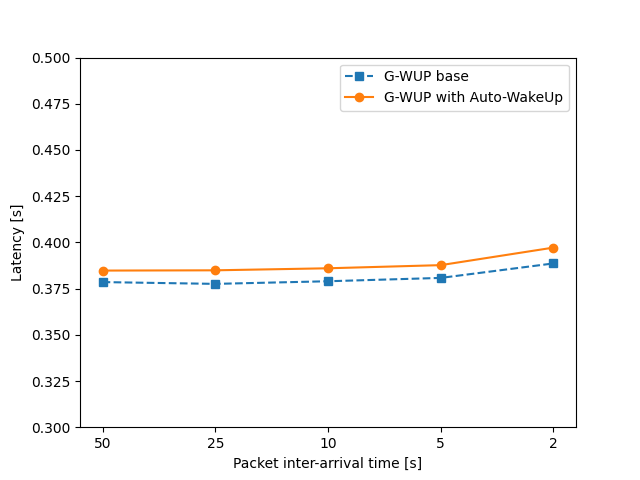
\includegraphics[width=1.1\linewidth]{Contents/Images/graphs/autoWakeUp/latency.png}
    \caption{End-to-End Latency}
    \label{fig:Latency_1}
  \end{subfigure}
  \begin{subfigure}[t]{0.49\linewidth}
    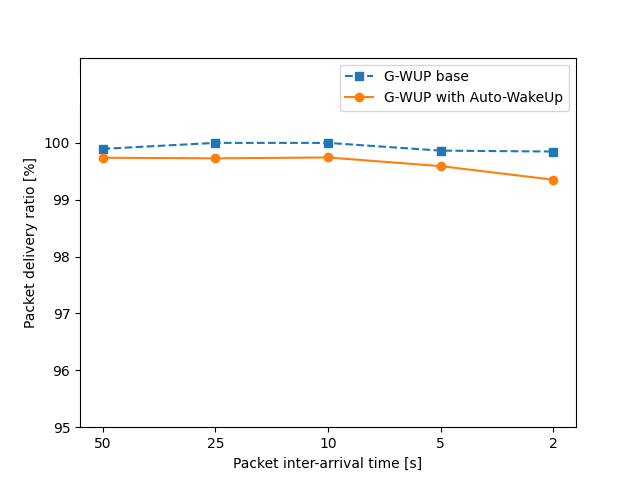
\includegraphics[width=1.1\linewidth]{Contents/Images/graphs/autoWakeUp/pdr.png}
    \caption{Packet Delivery Ratio}
    \label{fig:PDR_1}
  \end{subfigure}
  \caption{Confronto delle prestazioni tra versione base di GreenWUP (blu) e variante proposta (arancio) in termini di energia complessiva consumata, tempo in TX mode della WUR, latenza end-to-end e PDR}
  \label{fig:autoWakeUp}
\end{figure}

In sintesi, il meccanismo introdotto porta ad una ottimizzazione del tempo di trasmissione delle main radio ma non ha benefici significativi sulle
prestazioni end-to-end del sistema.
\newpage

\subsection{Relay-Caching}
Si precisa che tutti in tutti gli scenari simulati si assume che la rete sia completamente connessa per cui da un qualsiasi nodo \textit{x} è possibile raggiungere tramite uno o più nodi il nodo \textit{sink}.
\\\\
\textit{1) TX Time}: come mostrato in \textbf{Figura \ref{fig:TXTime_2}}, anche qui il tempo che in media i nodi utilizzano la wake-up Radio per trasmettere messaggi di wake-up diminuisce significativamente rispetto alla versione base di GreenWUP all'aumentare del traffico in rete. Questo è un risultato che ci si aspettava in quanto adesso i vari nodi hanno la possibilità di evitare lo scambio di pacchetti RTS/CTS con i propri vicini, che ricordiamo sono seguiti da messaggi di wake-up da e verso il nodo sender.\\
Ovviamente più pacchetti data vengono inviati e più volte si evita il classico scambio RTS/CTS, ecco perché questa variante presenta tempi in TX minori man mano che il traffico aumenta. In questo caso i miglioramenti sono tra il 50\% e il 62\%.
\\\\
\textit{2) Energy Consuption}: come mostrato in \textbf{Figura \ref{fig:EnergySpent_2}}, l'energia consumata dall'intera rete è minore rispetto l'energia consumata dalla versione base.\\
Anche in questo caso, il risultato è dovuto al fatto che ci sono molti meno scambi di RTS/CTS. In particolare questa procedura è eseguita soltanto una volta ogni quattro pacchetti data da inoltrare (dato che è possibile trasmettere verso il nodo cached per un massimo di 3 volte), inoltre, considerando che la procedura richiede l'invio di \(2 + ( 2 * n)\) pacchetti se si hanno \textit{n} possibili relay node che rispondo all' RTS del sender, è facile intuire un miglioramento nei consumi energetici di ogni nodo. I miglioramenti ottenuti sono, nel migliore dei casi (\textit{iaTime}=2), circa del 15\%. Per configurazioni con meno pacchetti si aggira invece intorno al 10-13\%.
\\\\
\textit{3) End-to-End Latency}: come mostrato in \textbf{Figura \ref{fig:Latency_2}}, non solo vi è un miglioramento rispetto la versione base di GreenWUP, ma questo fattore di miglioramento aumenta all'aumentare del traffico in rete.\\
Ovviamente questo è dovuto al fatto che in questo contesto, così come anche in altri, il concetto di \textit{caching} di informazioni dà il meglio di se in situazioni in cui il traffico è maggiore. Infatti non dovendo aspettare tempi\footnote{\'E stato citato il jitter randomico ma ovviamente ci sono anche altri tempi di attesa: ad esempio dopo l'invio di un messaggio di wake-up i nodi aspettano un tempo che permetta a chi riceve il messaggio di impostare la main radio in RX prima di mandare l'informazione.} come il jitter randomico, un nodo impiega molto meno tempo ad inoltrare un pacchetto verso un proprio vicino (se questo ovviamente è stato memorizzato in precedenza). I miglioramenti qui sono più importanti, infatti, abbiamo un miglioramento di circa il 25\% in reti molto trafficate che va a scendere fino a un minimo del 12-15\% per reti meno trafficate. 
\\\\
\textit{4) Packet Delivery Ratio}: come mostrato in \textbf{Figura \ref{fig:PDR_2}}, la percentuale di pacchetti ricevuti è paragonabile a quella della versione base, garantendo sempre la corretta ricezione di almeno il 99\% dei pacchetti.
\\\\
Ovviamente, come già detto, è molto importante per questa variante non "stressare" troppo i nodi cached in quanto se questi dovessero essere spesso non disponibili si andrebbero a fare svariate ritrasmissioni in più rispetto alla versione base, causando un degrado non sono in termini di latenza ma anche di energia consumata.\\
In questo caso, ogni nodo può trasmettere verso il nodo cached non più di 3 volte.

\begin{figure}[H]
  \begin{subfigure}[t]{0.49\linewidth}
    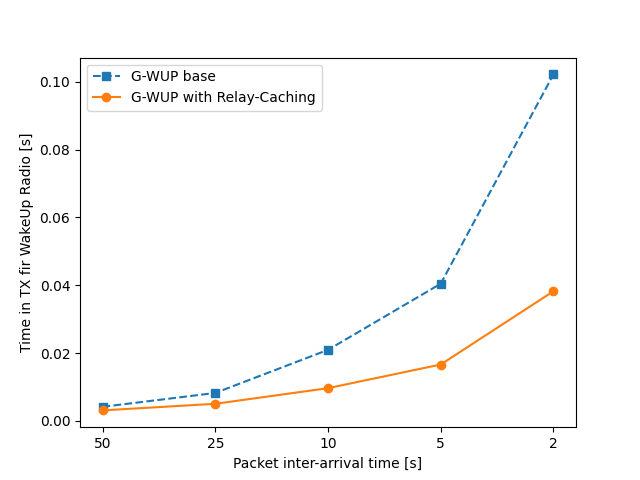
\includegraphics[width=1.1\linewidth]{Contents/Images/graphs/relayCaching/tx_time.png}
    \caption{TX Time for the WUR}
    \label{fig:TXTime_2}
  \end{subfigure}
  \begin{subfigure}[t]{0.49\linewidth}
    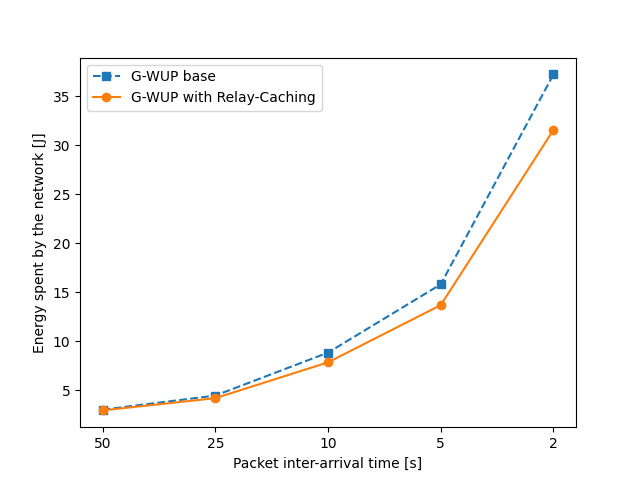
\includegraphics[width=1.1\linewidth]{Contents/Images/graphs/relayCaching/energySpent.png}
    \caption{Energy Consuption}
    \label{fig:EnergySpent_2}
  \end{subfigure}
  \begin{subfigure}[t]{0.49\linewidth}
    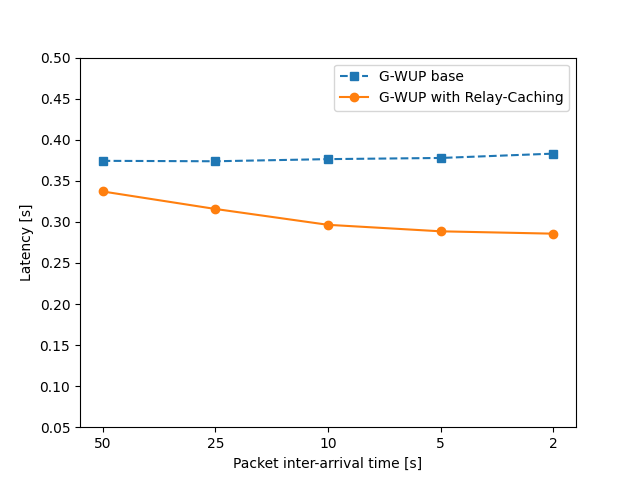
\includegraphics[width=1.1\linewidth]{Contents/Images/graphs/relayCaching/latency.png}
    \caption{End-to-End Latency}
    \label{fig:Latency_2}
  \end{subfigure}
  \begin{subfigure}[t]{0.49\linewidth}
    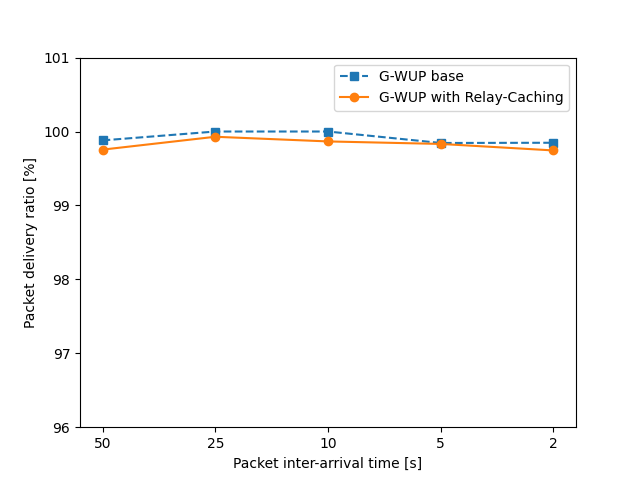
\includegraphics[width=1.1\linewidth]{Contents/Images/graphs/relayCaching/pdr.png}
    \caption{Packet Delivery Ratio}
    \label{fig:PDR_2}
  \end{subfigure}
  \caption{Confronto delle prestazioni tra versione base di GreenWUP (blu) e variante proposta (arancio)}
  \label{fig:relayCaching}
\end{figure}

In sintesi la variante che introduce il caching mostra di riuscire a ridurre significativamente il problema dell'attivazione della main radio con miglioramenti significativi in termini di energia consuma, senza degradare l'affidabilità della consegna delle informazioni. La variante riesce anche a ridurre in modo significativo le latenze, metrica importante in sistemi che, sempre piu', richiedono la rapida consegna di informazioni per supportare applicazioni "industria 4.0" o realizzare sistemi di allarme.

\subsection{All-in-One}
Si precisa che tutti in tutti gli scenari simulati si assume che la rete sia completamente connessa per cui da un qualsiasi nodo \textit{x} è possibile raggiungere tramite 1 o più nodi il nodo \textit{sink}.
\\\\
\textit{1) TX Time}: come mostrato in \textbf{Figura \ref{fig:TXTime_final}}, la versione che racchiude tutte le modifiche si comporta meglio rispetto alle altre soluzioni. Ovviamente in questo caso non solo si riduce di molto il numero di wake-up message scambiati durante la fase di relay selection, ma vengono meno tutti i wake-up message usati per sollecitare il nodo sender prima che i receiver inviino il pacchetto CTS.\\
Anche qui il coefficiente di miglioramento aumenta all'aumentare del numero di pacchetti DATA generata dai nodi della rete.\\
In particolare i miglioramenti sono del 77-80\% rispetto la versione base del protocollo GreenWUP e del 20-35\% rispetto ala variante con Auto-WakeUp.
\\\\
\textit{2) Energy Consuption}: come mostrato in \textbf{Figura \ref{fig:EnergySpent_final}}, c'è un piccolo miglioramento anche a livello di energia complessiva consumata dai nodi della rete. Ovviamente questo risultato era aspettato in quanto qui si sommano i vantaggi delle varianti di Relay-Selection e Auto-WakeUp in termini di invio di pacchetti (che siano questi di wake-up o RTS/CTS). Si ha infatti un piccolo miglioramento del 2-4\% rispetto la variante con Relay-Caching e un miglioramento totale di circa 15-18\% rispetto la versione base di GreenWUP.
\\\\
\textit{3) End-to-End Latency}: come mostrato in \textbf{Figura \ref{fig:Latency_final}}, nel caso della latenza quest'ultima variante si comporta praticamente come la versione con Relay-Caching tranne per qualche piccolo peggioramento in alcuni casi. \\
In particolare si ha un piccolo peggioramento che varia tra lo 0.5-1\% rispetto la versione con Relay-Caching mentre si ha un miglioramento del 20-26\% rispetto la versione base del protocollo GreenWUP. 
\\\\
\textit{4) Packet Delivery Ratio}: come mostrato in \textbf{Figura \ref{fig:PDR_final}}, vale quanto detto per la latenza end-to-end. Quest'ultima variante si comporta allo stesso modo della versione con Relay-Caching, presentando, di fatto, un piccolo peggioramento rispetto la versione base del protocollo GreenWUP base.\\
In particolare si ha un peggioramento dello 0.2\%, un peggioramento che non comporta grossi problemi, infatti, come tutte le altre varianti proposte, quest'ultima garantisce in media la carretta ricezione del 99.8\%.

\begin{figure}[H]
  \begin{subfigure}[t]{0.49\linewidth}
    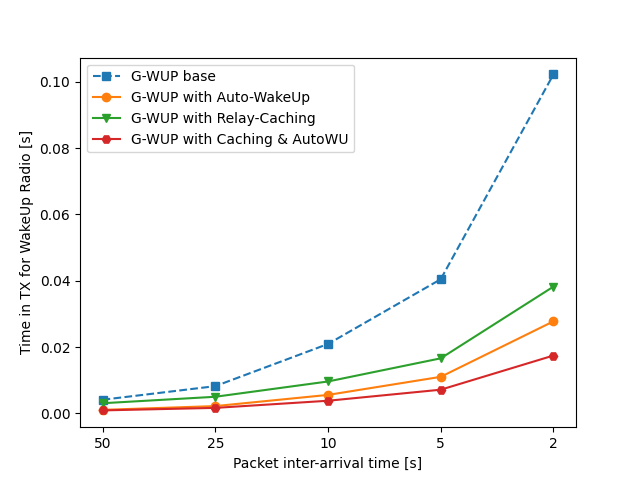
\includegraphics[width=1.1\linewidth]{Contents/Images/graphs/final/tx_time.png}
    \caption{TX Time for the WUR}
    \label{fig:TXTime_final}
  \end{subfigure}
  \begin{subfigure}[t]{0.49\linewidth}
    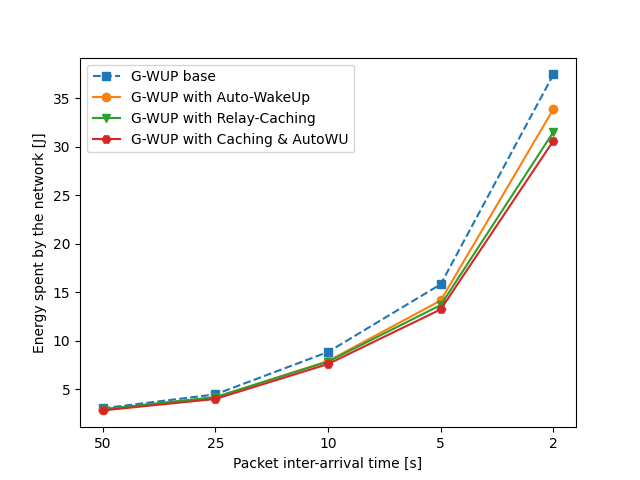
\includegraphics[width=1.1\linewidth]{Contents/Images/graphs/final/energySpent.png}
    \caption{Energy Consuption}
    \label{fig:EnergySpent_final}
  \end{subfigure}
  \begin{subfigure}[t]{0.49\linewidth}
    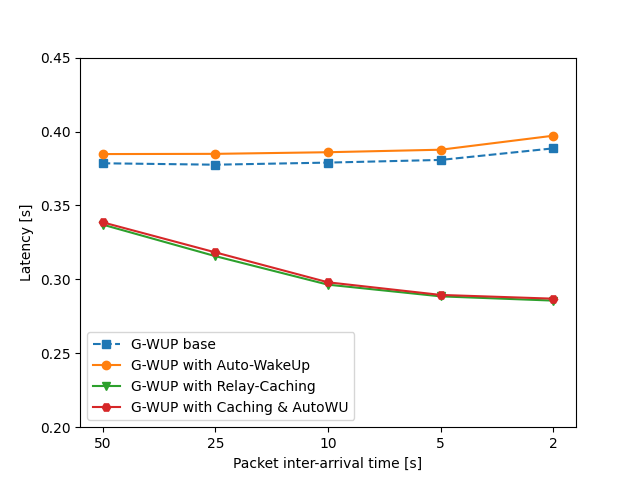
\includegraphics[width=1.1\linewidth]{Contents/Images/graphs/final/latency.png}
    \caption{End-to-End Latency}
    \label{fig:Latency_final}
  \end{subfigure}
  \begin{subfigure}[t]{0.49\linewidth}
    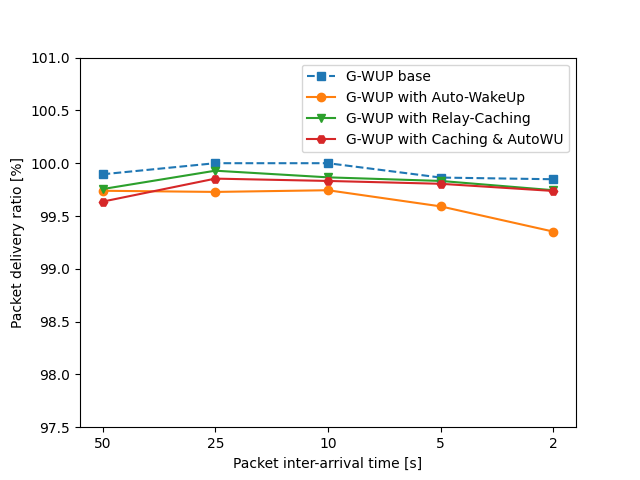
\includegraphics[width=1.1\linewidth]{Contents/Images/graphs/final/pdr.png}
    \caption{Packet Delivery Ratio}
    \label{fig:PDR_final}
  \end{subfigure}
  \caption{Confronto delle prestazioni tra versione base di GreenWUP (blu) e le varianti proposte}
  \label{fig:final}
\end{figure}

La versione All-in-One è quindi efficace nel ridurre la latenza e il consumo energetico di GreenWUP, ad un prezzo di un leggero degrado delle prestazioni in termini di packet delivery ratio.

\subsection{All-in-One 2.0}
Si precisa che tutti in tutti gli scenari simulati si assume che la rete sia completamente connessa per cui da un qualsiasi nodo \textit{x} è possibile raggiungere tramite uno o più nodi il nodo \textit{sink}.
\\\\
\textit{1) TX Time}: come mostrato in \textbf{Figura \ref{fig:TXTime_final2.0}}, si è riusciti a migliorare ulteriormente l'invio di pacchetti di wake-up rispetto la normale \textit{All-in-One}. Ovviamente questo miglioramento si ha in quanto essendo dinamico il tempo per cui si usa il caching di un relay e dato che il tetto massimo è maggiore del numero usato nella prima versione di \textit{All-in-One} ci saranno sicuramente meno fasi di Relay-Selection.\\
In particolare si osserva un miglioramento di circa il 47\% rispetto la prima versione di \textit{All-in-One}.
\\\\
\textit{2) Energy Consuption}: come mostrato in \textbf{Figura \ref{fig:EnergySpent_final2.0}}, la gestione dinamica del numero di ritrasmissioni e il Jitter basato sull'energia residua comportano un miglioramento anche nell'energia complessiva consumata dalla rete. Anche qui si ha un miglioramento del 5\% circa, dovuto al fatto che i vari nodi potrebbero evitare molte più volte la fase di Relay-Selection, avviandola solo nei casi in cui il nodo cached potrebbe scaricarsi.
\\\\
\textit{3) End-to-End Latency}: come mostrato in \textbf{Figura \ref{fig:Latency_final2.0}}, anche il ritardo End-to-End migliora rispetto la versione base. Ovviamente gestendo meglio l'energia consumata e non vincolando l'uso del nodo cached a 3 ma riducendolo o aumentandolo a seconda dei casi ci saranno meno ritrasmissioni dovuti a nodi non più disponibili oltre che meno scambi di pacchetti dovuti alla fase di Relay-Selection. \\
In particolare, anche qui, i miglioramenti sono circa del 5-6\% in tutte le varie configurazioni.
\\\\
\textit{4) Packet Delivery Ratio}: come mostrato in \textbf{Figura \ref{fig:PDR_final2.0}}, la percentuale dei pacchetti ricevuti, che era un punto debole della prima versione di \textit{All-in-One}, è migliorata molto. Si ottiene infatti sempre tra il 99.9\% e il 100\% dei pacchetti consegnati, perdendone circa in quantità minime come 2 o 3 solitamente. \\
Gestendo meglio l'energia ci saranno sempre meno nodi indisponibili per cui le probabilità di perdita dei pacchetti diminuiscono.

\begin{figure}[H]
  \begin{subfigure}[t]{0.49\linewidth}
    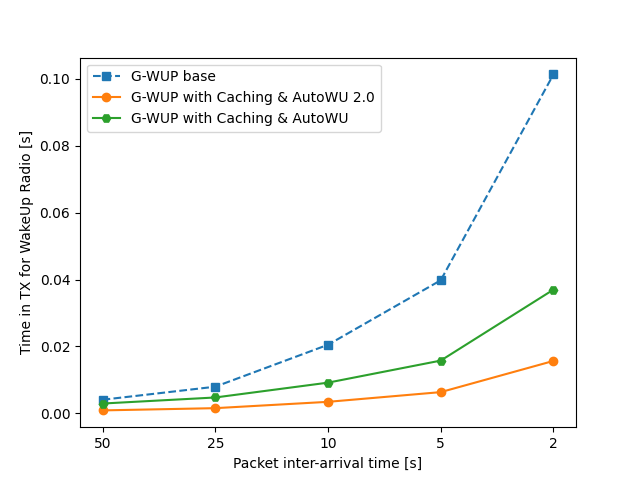
\includegraphics[width=1.1\linewidth]{Contents/Images/graphs/final2.0/tx_time.png}
    \caption{TX Time for the WUR}
    \label{fig:TXTime_final2.0}
  \end{subfigure}
  \begin{subfigure}[t]{0.49\linewidth}
    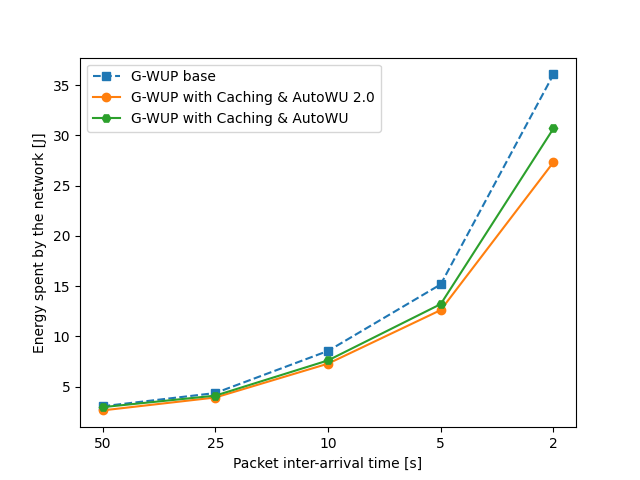
\includegraphics[width=1.1\linewidth]{Contents/Images/graphs/final2.0/energySpent.png}
    \caption{Energy Consuption}
    \label{fig:EnergySpent_final2.0}
  \end{subfigure}
  \begin{subfigure}[t]{0.49\linewidth}
    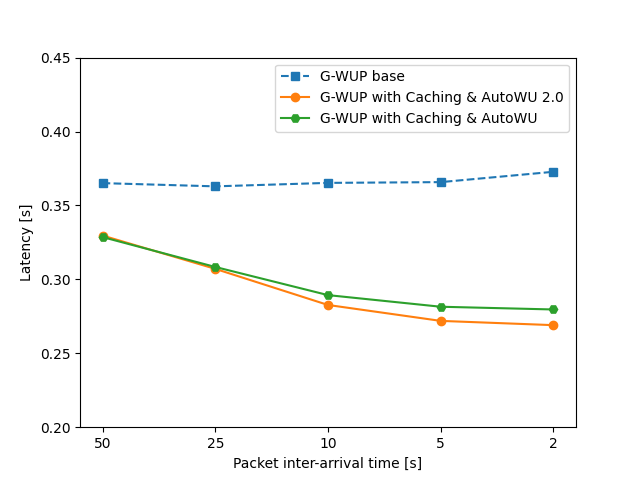
\includegraphics[width=1.1\linewidth]{Contents/Images/graphs/final2.0/latency.png}
    \caption{End-to-End Latency}
    \label{fig:Latency_final2.0}
  \end{subfigure}
  \begin{subfigure}[t]{0.49\linewidth}
    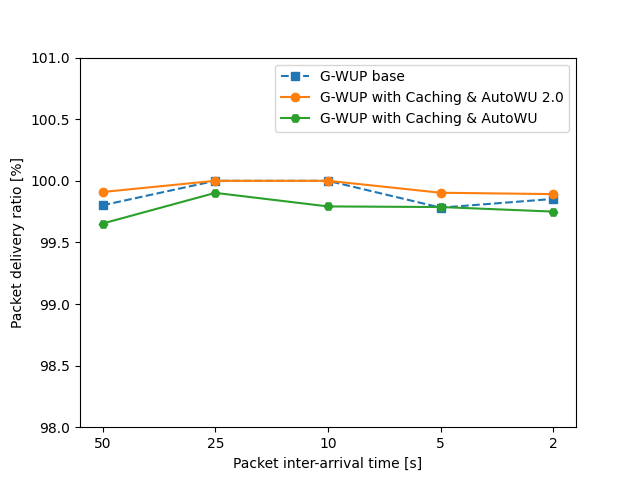
\includegraphics[width=1.1\linewidth]{Contents/Images/graphs/final2.0/pdr.png}
    \caption{Packet Delivery Ratio}
    \label{fig:PDR_final2.0}
  \end{subfigure}
  \caption{Confronto delle prestazioni tra versione base di GreenWUP (blu) e le varianti proposte}
  \label{fig:final2.0}
\end{figure}

La combinazione di tutti i meccanismi proposti consente netti miglioramenti in termini di tutte le metriche prestazionali rispetto al protocollo base. E' efficace nel ridurre al minimo gli onerosi scambi di pacchetti di controllo, consente la scelta dei migliori relay. Questo migliora le prestazioni in termini anche di packet delivery ratio e latenza.